\question In the figure below, two very long, thin wires run parallel to each other. A conventional current $I_1=0.3$ A flows through the bottom wire in the directions indicated. The loop in the wire has a radius $R=5$ cm, and the distance $d$ between the wires is 12 cm. What current $I_2$ is required in the top wire (both direction and magnitude) in order to cancel the magnetic field at the center of the loop?

\begin{figure}[ht!]
	\centering
	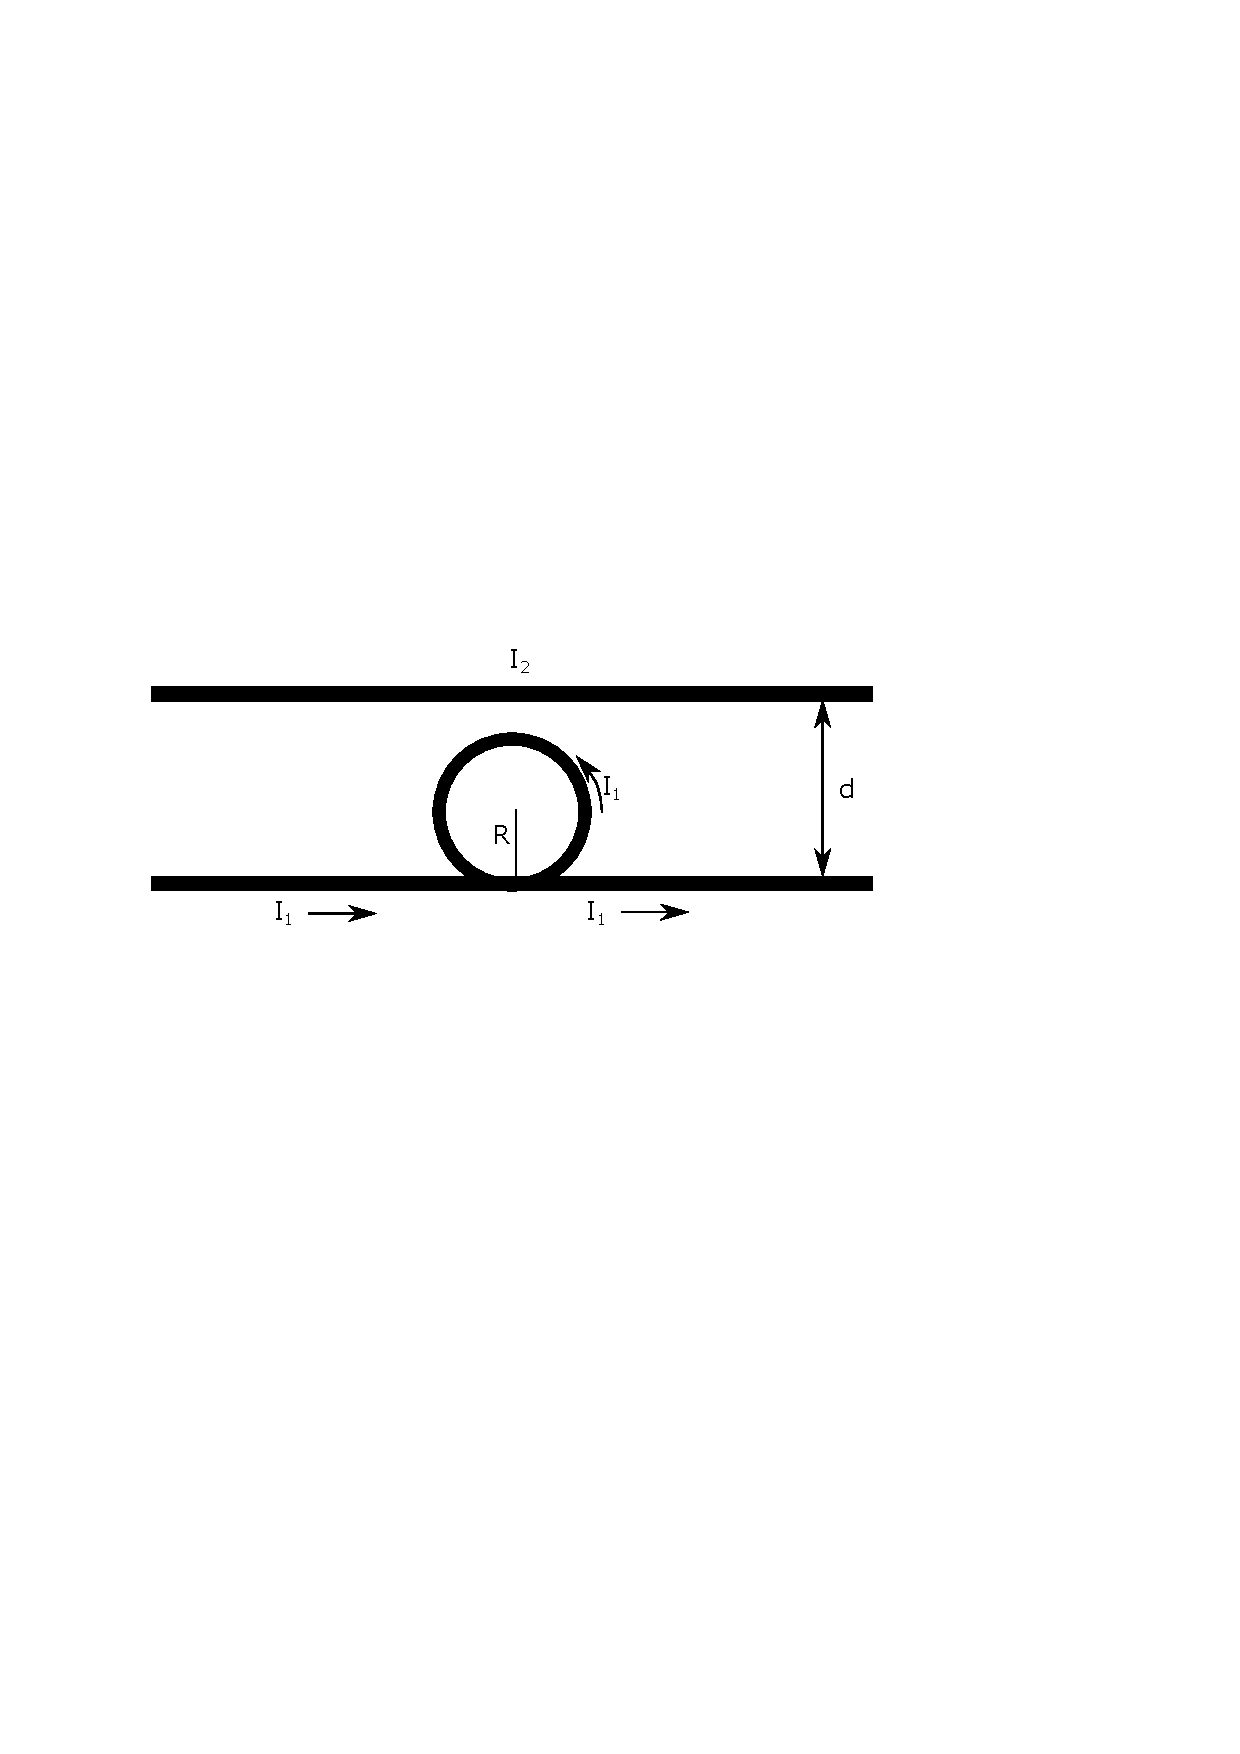
\includegraphics[width=8cm]{bfield_exam2.pdf}
\end{figure}